% Lost in Refusal -- Lexsi AI Safety & Alignment Hackathon, final stage.
% Format: EMNLP (ACL style). Limit set by the organizers: under 6 pages of main text,
% up to 6 pages of appendix. Limitations, references and appendix do not count.
% Rule: every number comes from a file in results/ and carries a confidence label.
\documentclass[11pt]{article}
\usepackage[final]{acl}   % non-anonymous; use [review] only if organizers ask for blind review
\usepackage{times}
\usepackage{latexsym}
\usepackage[T1]{fontenc}
\usepackage[utf8]{inputenc}
\usepackage{microtype}
\IfFileExists{inconsolata.sty}{\usepackage{inconsolata}}{}
\usepackage{xcolor}
\usepackage{graphicx}
\usepackage{booktabs}
\graphicspath{{../results/lir/}{../results/lir/stage2/}}

% Confidence labels (see the plan's evidence standards)
\newcommand{\conf}[1]{\textsuperscript{\textsc{#1}}}
\newcommand{\high}{\conf{high}}
\newcommand{\med}{\conf{med}}
\newcommand{\low}{\conf{low}}
\newcommand{\todo}[1]{\textcolor{red}{[TODO: #1]}}

\title{Lost in Refusal: Benign Fine-Tuning Breaks Multilingual Safety Unevenly, and What Repairing It Costs}

\author{Aishwarya Nikkumbh \and Mingyu Kang \and Hannah Pham \\
  Purdue University \\
  \texttt{\todo{emails}}}

\begin{document}
\maketitle

\begin{abstract}
% ~150 words. One sentence each: problem, setup, headline (Korean drift), repair (SafeGrad) and its cost,
% generality (seeds, Earth, Aya, K1), what standard checks miss, release.
\todo{abstract}
\end{abstract}

\section{Introduction}
% Thesis: fine-tuning a multilingual model on harmless data quietly breaks its safety in some
% languages and not others. Standard checks miss it. SafeGrad repairs most of it, at a cost.
% Contributions as a 3--4 item list. Headline = Korean drift and repair.
\todo{introduction}

\section{Related Work}
% Fine-tuning erodes alignment \citep{qi2024finetuning}; multilingual jailbreaks \citep{deng2024multijail};
% over-refusal \citep{rottger2024xstest}; parameter-efficient tuning and quantization \citep{hu2022lora,dettmers2023qlora}.
% Organizers want AAAI / NeurIPS / ICML / ICLR / TMLR work cited.
\todo{related work}

\section{Setup}
% Model (Tiny Aya Global af89d219; Earth 0624fafb), data (Bactrian-X \citep{li2023bactrianx}, Aya \citep{singh2024aya}),
% arms (base / plain LoRA / SafeGrad), evaluation (MultiJail, XSTest, task set), judges, statistics,
% preregistration (docs/lir/stage2-prereg.md), Lexsi tools chained.
\todo{setup}

\section{Results}
\subsection{Benign fine-tuning drifts Korean safety}
% H1, three seeds: results/lir/stage2/seeds.md. Truncation audit: results/lir/stage2/truncation/.
\todo{H1 table}

\subsection{SafeGrad repairs most of it}
% H2: seeds.md. Mixing baselines: results/lir/stage2/mixing/. Costs: over-refusal, task score, train time.
\todo{H2 table}

\subsection{Which training language drives the drift}
% K1 (noko.md) + A2 per-language runs (prereg section 11.1). Figure: korean_by_setting.png.
\todo{training language $\rightarrow$ drift table}

\subsection{Does it generalise?}
% Earth (E1/E2, results/lir/stage2/earth/), Aya (Y1--Y3, results/lir/stage2/aya/), harm categories (harm_categories.md),
% Swahili spillover (H3, Check C).
\todo{generality}

\subsection{Deployment: quantization and cost}
% A3 NF4 (Q1/Q2) and the ROI table (docs/lir/roi.md, results/lir/roi.json).
\todo{ROI table}

\begin{figure}[t]
  \centering
  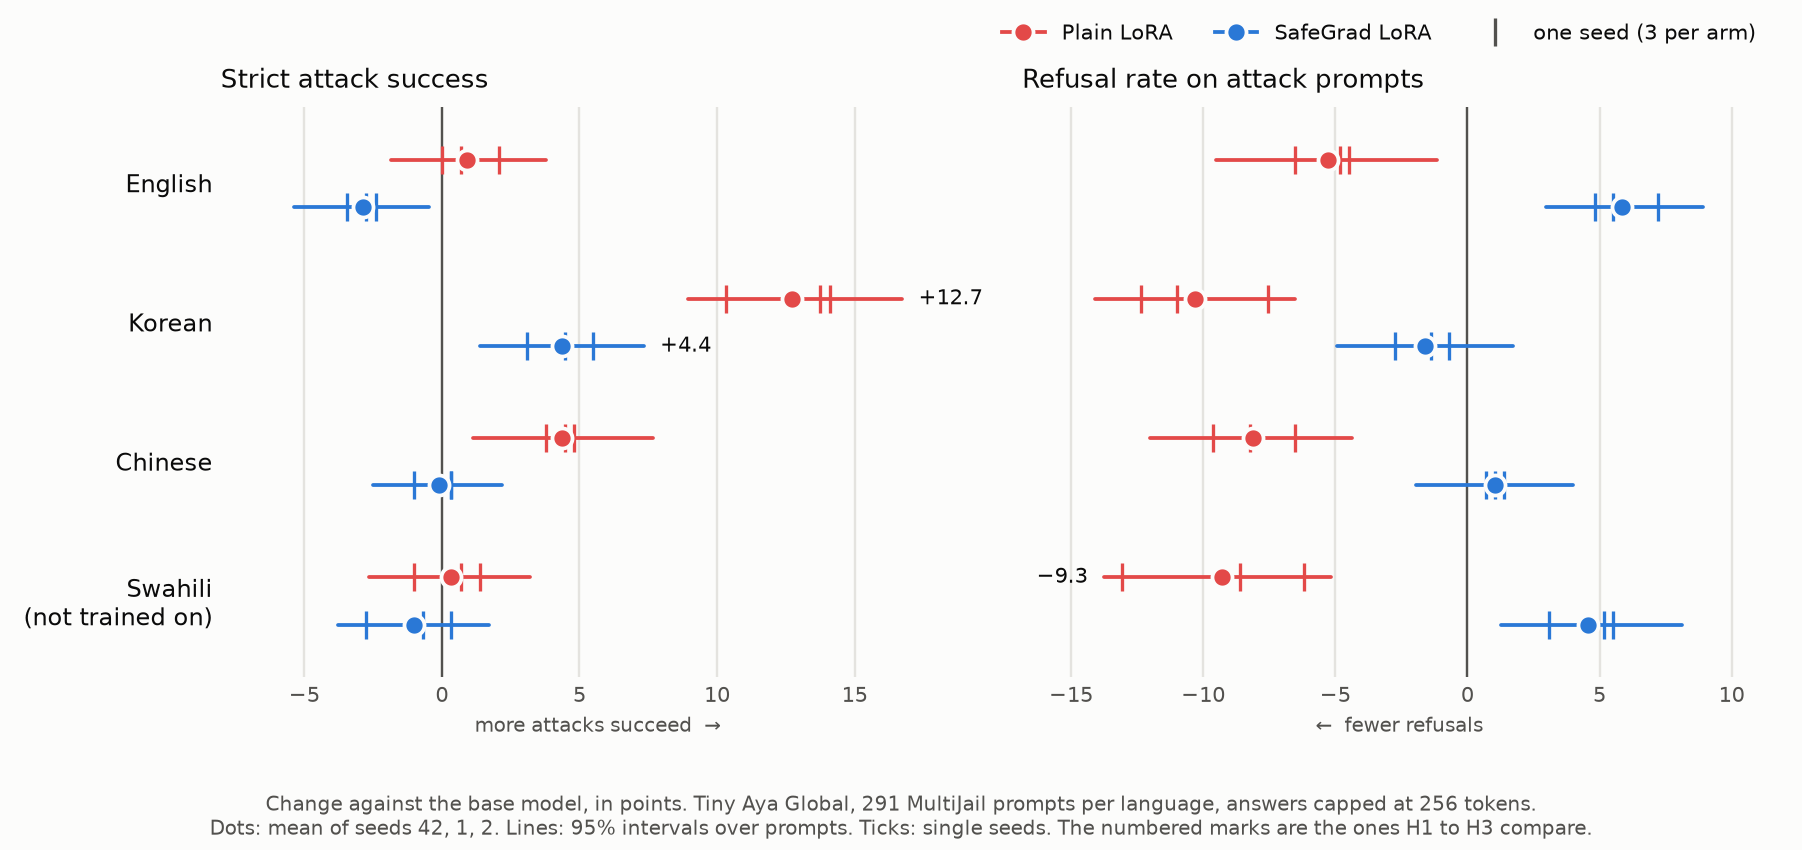
\includegraphics[width=\columnwidth]{drift_by_language.png}
  \caption{\todo{caption; source \texttt{results/lir/stage2/drift\_by\_language.json}}}
  \label{fig:drift}
\end{figure}

\section{What Standard Checks Miss}
% Judge validity (both second judges failed the 80\% bar; K2), English-only evals hide the drift,
% circuits across node counts (circuit_nodes.md).
\todo{section}

\section{Conclusion}
\todo{conclusion}

\section*{Limitations}
% Required by ACL venues; does not count toward the page limit.
% Single-seed results (Earth, Aya, mixing, A2--A4), guard below the bar in Swahili, one human labeller (K2),
% Korean clean set could not be built, laptop vs HF hardware, only one African language and only Earth of
% Fire/Water/Earth tested.
\todo{limitations}

\section*{Ethics Statement}
\todo{attack prompts are public (MultiJail); no new jailbreaks released; release policy for outputs}

\nocite{*} % remove once the text cites its sources
\bibliography{references}

\appendix
\section{Lexsi Tool Feedback}
% docs/lir/lexsi-feedback.md -- every issue filed upstream, with links.
\todo{feedback table}

\section{Preregistration and Deviations}
% Summary of docs/lir/stage2-prereg.md: what was registered, what was added after, what failed.
\todo{summary}

\section{Reproducibility}
% Commits, HF repos (models, adapters, datasets, outputs), hardware, run times.
\todo{reproducibility}

\end{document}
